\documentclass{article}
\usepackage{amsmath}
\usepackage{tikz}
\usepackage{hyperref}
\usepackage[a4paper]{geometry}
\usepackage{fancyhdr}
\pagestyle{fancy}
\lhead{Aufladeprozess eines Kondensators}
\rhead{August 2025}
\begin{document}
\section{Aufladeprozess eines Kondensators}
Beim Aufladen eines Kondensators wird es mit der Zeit schwerer weitere Ladungen auf den Kondensator zu übertragen, je geladener dieser bereits ist. Somit ist die Ladungsgeschwindigkeit, $I(t)$, bei $t=0$ das eigene Maximum, $I_0$, bevor sie \hyperref[Wachstumsfunktionen]{exponentiell zu $0$ zerfällt}. Genauso steigt die Spannung anfangs schnell bevor sie sich an $U_0$ annähert. Somit kann dies als begrenztes Wachstum dargestellt werden. \newline
Beim Entladen gilt eigentlich einfach nur das Gegenteil. Die Stromstärke verhält sich eigentlich so wie beim Aufladen, nur dass der Strom in die entgegengesetzte Richtung fließt, also negativ ist. Die bereits geladene Spannung zerfällt exponentiell zu $0$.
 
\subsection{Formeln}
Beim Aufladeprozess gilt \newline 
\begin{minipage}{0.5\linewidth}
 \center
 $I(t)=I_0 \cdot e^{-kt}$
 
 \begin{tikzpicture}
  \draw[->, domain=0:4, blue] plot ({\x}, {2.5*e^(-1.5*\x)}); 
  \draw[thick, ->] (0, 0) -- (4, 0) node[right] {$t$};
  \draw[thick, ->] (0, 0) -- (0, 2.5) node[above] {$I$};
 \end{tikzpicture} 
\end{minipage}
\hfill
\begin{minipage}{0.5\linewidth}
 \center
 $U(t)=U_0 - U_0 \cdot e^{-kt}$
 
 \begin{tikzpicture}
  \draw[->, domain=0:4, blue] plot ({\x}, {2.5 - 2.5*e^(-1.5*\x)}); 
  \draw[thick, ->] (0, 0) -- (4, 0) node[right] {$t$};
  \draw[thick, ->] (0, 0) -- (0, 2.5) node[above] {$U$};
 \end{tikzpicture}
\end{minipage} 
 
\vspace*{2\baselineskip} 
\noindent Beim Entladeprozess gilt \newline 
\begin{minipage}{0.5\linewidth}
 \center
 $I(t)=-I_0 \cdot e^{-kt}$
 
 \begin{tikzpicture}
  \draw[->, domain=0:4, blue] plot ({\x}, {-2.5*e^(-1.5*\x)}); 
  \draw[thick, ->] (0, 0) -- (4, 0) node[right] {$t$};
  \draw[thick, ->] (0, 0) -- (0, -2.5) node[below] {$I$};
 \end{tikzpicture} 
\end{minipage}
\hfill
\begin{minipage}{0.5\linewidth}
 \center
 $U(t)=U_0 \cdot e^{-kt}$
 
 \begin{tikzpicture}
  \draw[->, domain=0:4, blue] plot ({\x}, {2.5*e^(-1.5*\x)}); 
  \draw[thick, ->] (0, 0) -- (4, 0) node[right] {$t$};
  \draw[thick, ->] (0, 0) -- (0, 2.5) node[above] {$U$};
 \end{tikzpicture} 
\end{minipage}  
  
\subsection{Messen}
\begin{minipage}{\dimexpr\linewidth-4cm}
Die zurzeitige Stromstärke und Spannung bei Auf- und Entladen eines Kondensators kann durch ein Stromkreis wie dem hier rechts dargestellten gemssen werden. \newline
Durch das Umstellen des Schalters kann ein Stromkreis zwischen der Stromquelle, dem Kondensator und allem dazugehörigen aufgestellt werden, so dass dieser aufgeladen wird. Wird der Schalter auf die andere Seite umgestellt, so besteht kein Stromkreis zwischen der Stromquelle und dem Kondensator mehr, nur noch einer zwischen dem Kondensator und dem Widerstand und den Messgeräten, so dass der Kondensator entladen wird. 
\end{minipage}
\hfill
\begin{minipage}{4cm}
 \center
 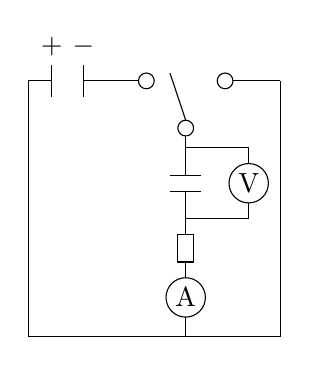
\begin{tikzpicture}
  \draw (0.2, -0.2) -- (0.2, 0.2) node[above] {$-$};
  \draw (-0.2, -0.2) -- (-0.2, 0.2) node[above] {$+$};
 
  \draw (-0.2, 0) -- (-0.5, 0);
  \draw (-0.5, 0) -- (-0.5, -3.25);
  \draw (0.2, 0) -- (0.9, 0);
  \draw (1, 0) circle (0.1); 
  
  \draw (1.5, -0.5) -- (1.3, 0.1); 
  \draw (1.5, -0.6) circle (0.1); 
  \draw (1.5, -0.7) -- (1.5, -1.2);
  \draw (1.3, -1.2) -- (1.7, -1.2);
  \draw (1.3, -1.4) -- (1.7, -1.4);
  \draw (1.5, -0.85) -- (2.3, -0.85);
  \draw (2.3, -0.85) -- (2.3, -1.05);
  \draw (2.3, -1.3) circle (0.25) node {V};
  \draw (2.3, -1.55) -- (2.3, -1.75);
  \draw (2.3, -1.75) -- (1.5, -1.75);
  \draw (1.5, -1.4) -- (1.5, -1.95);
  \draw (1.4, -1.95) rectangle (1.6, -2.3);
  \draw (1.5, -2.3) -- (1.5, -2.5);
  \draw (1.5, -2.75) circle (0.25) node {A};
  \draw (1.5, -3) -- (1.5, -3.25);
 
  \draw (2, 0) circle (0.1);
 
  \draw (2.1, 0) -- (2.7, 0);  
  \draw (2.7, 0) -- (2.7, -3.25);
  \draw (-0.5, -3.25) -- (2.7, -3.25);
 \end{tikzpicture} 
\end{minipage}  
 
\subsection{Funktionen Bestimmen}
Ein Funktion $I(t)$ oder $U(t)$ kann anhand gegebener Messdaten bestimmt werden, indem eine \hyperref[Umgang mit dem Taschenrechner in Physik]{Exponential-Regression} durchgeführt wird. Aufgrund der obigen begründungen kann die Funktion offensichtlich nicht konstant oder zu $t$ proportional sein, sondern muss in einer Form antiproportional sein. Obwohl $f(t)=t^a$ mit $a < 0$ einer ähnlichen Form folgen kann, kann es nicht für $I(t)$ oder $U(t)$ genutzt werden, weil hier $f(0)$ undefiniert ist, diese aber definiert, als $I_0$ beziehungsweise $U_0$, sein müssen.
 
\subsection{Halbwertzeit}
Der Faktor $k$ der e-Funktionen kann auch als $\dfrac{1}{RC}$ aufgeschrieben werden. Aus weiteren Umformungen folgt dass für eine Funktion $f(t)$ des exponentiellen Zerfalls die Halbwertzeit bei $t = \ln{(2)} \cdot RC$ erreicht, so dass also $f(\ln{(2)} \cdot RC) = \dfrac{1}{2} f(0)$. 
\end{document}